\subsection{Le modèle de mobilité}

Un modèle de mobilité a été mis en place dans Blue Banana, nous allons le présenter car il est utilisé pour les différents tests réalisés pour les solutions mises en place. Pour cela, un degré de mobilité à un instant donné, a été introduit. Il s'agit du nombre d'avatars dans l'état \textbf{T}(ravelling) à cet instant sur le nombre total d'avatars. Le modèle de mobilité implémenté dans Blue Banana se base sur l'automate (cf partie~\ref{Automate}). A intervalles réguliers, PeerSim décide si un avatar doit ou non changer d'état. Il réalise ceci grâce aux différentes probabilités présentées dans les fichiers de configurations. A chaque fois qu'un déplacement est décidé, une destination est choisie. L'avatar commence alors son déplacement, chaque mouvement est rectiligne mais non uniforme (car accélération). L'accélération est nulle lorsque la vitesse maximale est atteinte, cette vitesse maximale est choisie en fonction de la zone où se trouve l'avatar.


\par L'automate étant mis à jour toutes les 100ms, même un petit changement dans les probabilités, peut entrainer des gros changements sur la mobilité. La transition WtoT a été choisie, dans Blue Banana, pour faire varier la mobilité. Cette transition permet de déclencher le passage d'un avatar d'un état d'exploration désordonné à un état de déplacement rapide. Sur la figure~\ref{fig:mobility}, nous pouvons voir les différentes valeurs affectées à la transition et les degrés de mobilité correspondants. 

\begin{figure}
  \begin{center}
    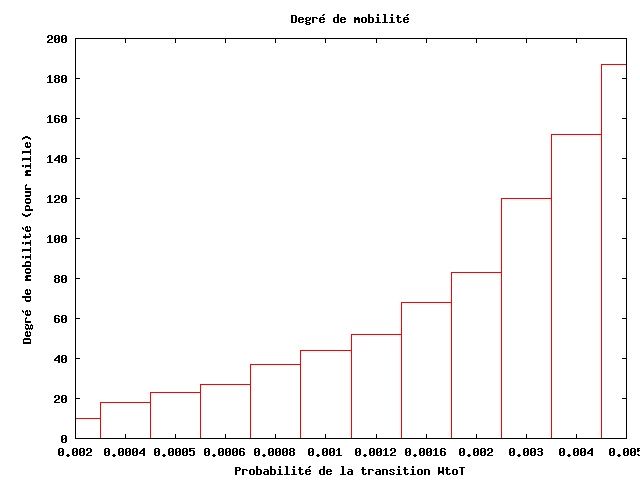
\includegraphics[scale=0.40]{./Ressources/Images/mobility.png} \\
    \caption{\textit{\small Influence du changement de probabilité sur
        la transition WtoT de l'automate sur le degré de mobilité du
        Métavers}}
    \label{fig:mobility}
  \end{center}
\end{figure}


